%!TEX root = ./Basilisk-SPACECRAFTPLUS-20170808.tex


\section{Model Description}

\subsection{Introduction}

SpacecraftPlus is an instantiation of the dynamicObject abstract class. This abstract class is representing systems that have equations of motion that need to be integrated and therefore the main goal of this dynamic object is finding the state derivatives and interfacing with the integrator to integrate the state forward in time. SpacecraftPlus is representing a spacecraft that can be simulating only the translational movement which would mean the spacecraft only has mass (for gravity only simulations, setting the mass is not necessary), it could be simulating only rotational dynamics which would result in the spacecraft only having inertia, and finally both translational and rotational dynamics can be simulated at a time which results in the spacecraft having mass, inertia and center of mass offset.

SpacecraftPlus is the module where the equations of motion of the spacecraft are computed including the interaction between the hubEffector, stateEffectors and dynamicEffectors. The hubEffector is where the translational and rotational state derivatives are computed, the stateEffectors give contributions to spacecraftPlus and computes their own derivatives and the dynamcEffectors provide force and torque contributions to spacecraftPlus.

To give more description on this complex relationship, Figure~\ref{fig:FlexSloshFigure} shows an example of a spacecraft with a fuel slosh particle and a couple hinged rigid bodies connected to it. From a spacecraftPlus perspective there are some important variables and frame definitions needed to be defined. The body frame, \frameDefinition{B}, is a Cartesian reference frame that is fixed to the hub (the rigid body of the spacecraft) with no constraints on its orientation with respect to the hub. Additionally its origin, $B$, can be placed anywhere on the hub. The inertial frame, \frameDefinition{N}, is the inertial reference frame used in the formulation of the dynamics. The hub has some remaining variables needed to be defined which are the mass of the hub, $m_{\textnormal{hub}}$, center of mass of the hub location, $B_c$, and the inertia of the hub about its center of mass, $[I_{\textnormal{hub},B_c}]$. 

More variables needed to be defined for the spacecraftPlus, are the total mass of the spacecraft, $m_{\textnormal{sc}}$, the total inertia of the spacecraft about point $B$,  $[I_{\textnormal{sc},B}]$ and the center of mass location with respect to point $B$ vector, $\bm c$. Additionally, the state variables for the hub are $\bm r_{B/N}$, $\dot{\bm r}_{B/N}$, $\bm \sigma_{\cal{B}/\cal{N}}$ and $\bm \omega_{\cal{B}/\cal{N}}$, which are the position and velocity of point $B$ with respect to $N$ which describes the translational motion of the spacecraft, the MRP set for the orientation of $\cal{B}$ with respect to $\cal{N}$, and the angular velocity of the $\cal{B}$ with respect to $\cal{N}$ with describes the rotation of the spacecraft, respectively. 


\begin{figure}[htbp]
	\centerline{
		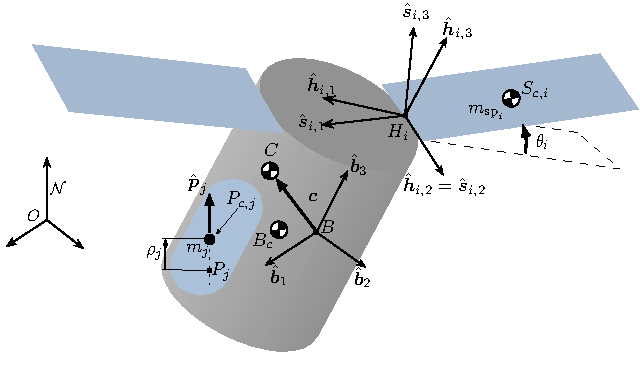
\includegraphics[width=0.8\textwidth]{Figures/Flex_Slosh_Figure}}
	\caption{Complex spacecraft that can be simulated using spacecraftPlus}
	\label{fig:FlexSloshFigure}
\end{figure}

\subsection{Equations of Motion}

The main description that is needed for spacecraftPlus are the equations of motion (EOMs). The following equation describes the translational EOM if only translation is enabled. This is Newton's Second Law on the center of mass of the spacecraft but when translation only is enabled the center of mass of the spacecraft is coincident with point $B$. 

\begin{equation}
m_{\text{sc}} \ddot{\bm r}_{B/N} = m_{\text{sc}} \ddot{\bm r}_{C/N} =  \bm F_{\textnormal{ext}}
\label{eq:Rbddot3}
\end{equation}

The following equation describes the rotational EOM if only rotational is enabled. This is similar to what can be seen in Reference~\cite{schaub} 
\begin{equation}
\Big[[I_{\text{sc},B}]+\sum\limits_{i=1}^{N} [D_{\textnormal{contr},i}]\Big] \dot{\bm\omega}_{\cal B/N} = - [\bm{\tilde{\omega}}_{\cal B/N}] [I_{\text{sc},B}] \bm\omega_{\cal B/N} + \bm{L}_B +\sum\limits_{i=1}^{N} \bm v_{\textnormal{rot,contr},i}
	\label{eq:Final6}
\end{equation}
$[D_{\textnormal{contr},i}]$ and $\bm v_{\textnormal{rot},i}$ will be defined in the next set of equations. 

Finally, the two following equations describe the translational and rotational EOMs when the both rotational and translational equations are enabled. 

\begin{multline}
\Big(m_{\text{sc}} [I_{3\times3}] +\sum_{i=1}^{N}[A_{\textnormal{contr},i}]\Big)\ddot{\bm r}_{B/N}+\Big(-m_{\text{sc}} [\tilde{\bm{c}}] +\sum_{i=1}^{N}[B_{\textnormal{contr},i}]\Big) \dot{\bm\omega}_{\cal B/N} \\
= \bm F_{\textnormal{ext}} 	- 2 m_{\text{sc}} [\tilde{\bm\omega}_{\cal B/N}] \bm c'
-m_{\text{sc}} [\tilde{\bm\omega}_{\cal B/N}][\tilde{\bm\omega}_{\cal B/N}]\bm{c}
+\sum_{i=1}^{N}\bm v_{\textnormal{trans,contr},i}
\label{eq:Rbddot8}
\end{multline}

\begin{multline}
\Big[m_{\text{sc}}[\tilde{\bm{c}}] +\sum\limits_{i=1}^{N}[C_{\textnormal{contr},i}]\Big]\ddot{\bm r}_{B/N}+\Big[[I_{\text{sc},B}]+\sum\limits_{i=1}^{N}[D_{\textnormal{contr},i}]\Big]\dot{\bm\omega}_{\cal B/N}
\\
= -[\bm{\tilde{\omega}}_{\cal B/N}] [I_{\text{sc},B}] \bm\omega_{\cal B/N} 
- [I'_{\text{sc},B}] \bm\omega_{\cal B/N} + \bm{L}_B +\sum\limits_{i=1}^{N}\bm v_{\textnormal{rot,contr},i}
\label{eq:Final9}
\end{multline}	
Where $[A_{\textnormal{contr},i}]$, $[B_{\textnormal{contr},i}]$, $[C_{\textnormal{contr},i}]$, $[D_{\textnormal{contr},i}]$, $\bm v_{\textnormal{trans,contr},i}$, and $\bm v_{\textnormal{rot,contr},i}$, are the contributions from the stateEffectors using the back-substitution method seen in Reference~\cite{Allard2016rz} and also discussed more in detail in the hinged rigid body state effector document.

The equations can now be organized into the following matrix representation:

\begin{equation}
\begin{bmatrix}
[A] & [B]\\
[C] & [D]
\end{bmatrix} \begin{bmatrix}
\ddot{\bm r}_{B/N}\\
\dot{\bm\omega}_{\cal B/N}
\end{bmatrix} = \begin{bmatrix}
\bm v_{\text{trans}}\\
\bm v_{\text{rot}}
\end{bmatrix}
\label{eq:backSub}
\end{equation}
And are solved using the following equations:
\begin{equation}
\dot{\bm\omega}_{\cal B/N} = \Big([D] - [C]][A]^{-1}[B]\Big)^{-1}(\bm v_{\text{rot}} - [C][A]^{-1}\bm v_{\text{trans}})
\end{equation}
\begin{equation}
\ddot{\bm r}_{B/N} = [A]^{-1} (\bm v_{\text{trans}} - [B]\dot{\bm\omega}_{\cal B/N})
\end{equation}
This shows that only two $3\times 3$ matrices are needed to solve this system of equations. One remaining equation that should be included is the kinematic relationship between $\bm \sigma_{\cal{B}/\cal{N}}$ and $\bm \omega_{\cal{B}/\cal{N}}$. This relationship can be seen in the following equation:

\begin{equation}
\dot{\bm \sigma}_{\cal{B}/\cal{N}} = \frac{1}{4} [B(\bm \sigma)]\bm \omega_{\cal{B}/\cal{N}}
\end{equation}
Where the full definition of $[B(\bm \sigma)]$ can be seen in Reference~\cite{schaub}. The kinematic relationship between $\bm r_{B/N}$ and $\dot{\bm r}_{B/N}$ is trivial because the inertial time derivative of $\bm r_{B/N}$ is equal to $\dot{\bm r}_{B/N}$. This completes the necessary equations needed for discussion on the EOMs of the system.

\subsection{Energy and Momentum Calculations}

A key part of spacecraftPlus is finding the total energy and momentum of the spacecraft for validation purposes. This section describes how the energy and momentum is calculated in spacecraftPlus.

\subsubsection{Total Orbital Kinetic Energy}

The total orbital kinetic energy (i.e. kinetic energy of the center of mass) of the spacecraft is
\begin{equation}
T_{\text{orb}} = \frac{1}{2} m_{sc} \dot{\bm r}_{C/N} \cdot \dot{\bm r}_{C/N}
\end{equation}
Expanding $\dot{\bm r}_{C/N}$ to be in terms of $\dot{\bm r}_{B/N}$ and $\dot{\bm c}$ results in
\begin{equation}
T_{\text{orb}} = \frac{1}{2} m_{sc} (\dot{\bm r}_{B/N} + \dot{\bm c}) \cdot (\dot{\bm r}_{B/N} + \dot{\bm c})
\end{equation}
Which simplifies to final desired equation
\begin{equation}
T_{\text{orb}} = \frac{1}{2} m_{sc} (\dot{\bm r}_{B/N}\cdot \dot{\bm r}_{B/N} + 2 \dot{\bm r}_{B/N} \cdot \dot{\bm c} + \dot{\bm c} \cdot \dot{\bm c})
\end{equation}

\subsubsection{Total Orbital Potential Energy}

The total orbital potential energy depends on what type of gravity model you are using. For simplicity, the orbital potential energy due to point gravity is included here but would need to be changed for spherical harmonics, etc. 

\begin{equation}
V_{\text{orb}} = \frac{\mu}{\vert \bm r_{C/N} \vert}
\end{equation}

\subsubsection{Total Orbital Energy}

Since the total orbital energy of the spacecraft must be conserved when there are no non-conservative external forces and torques acting on the spacecraft, it convenient to combine the kinetic and potential energies into one term, $E_{\text{orb}}$. This can be seen in the following equation.

\begin{equation}
E_{\text{orb}} = T_{\text{orb}} - V_{\text{rot}}
\end{equation}

\subsubsection{Total Rotational and Deformational Kinetic Energy}

The total rotational and deformational kinetic energy (i.e. kinetic energy about the center of mass) of the spacecraft is
\begin{multline}
T_{\text{rot}} = \frac{1}{2} \bm \omega_{\cal{B/N}}^T [I_{\text{hub},B_c}] \bm \omega_{\cal{B/N}} + \frac{1}{2} m_{\text{hub}} \dot{\bm r}_{B_c/C} \cdot \dot{\bm r}_{B_c/C} \\
+ \sum\limits_{i}^{N}\Big(\frac{1}{2} \bm \omega_{\cal{E}_{\textit{i}}/\cal{N}}^T [I_{\text{eff},E_{c,i}}] \bm \omega_{\cal{E}_{\textit{i}}/\cal{N}}
+ \frac{1}{2} m_{\text{eff}} \dot{\bm r}_{E_{c,i}/C} \cdot \dot{\bm r}_{E_{c,i}/C}\Big)
\end{multline}
Where $N$ is the number of state effectors attached to the hub, ``eff" is the current state effector which a frame specified as $\cal{E}_{\textit{i}}$ and a center of mass location labeled as point $E_{c,i}$. Expanding these terms similar to orbital kinetic energy results in 
\begin{multline}
T_{\text{rot}} = \frac{1}{2} \bm \omega_{\cal{B/N}}^T [I_{\text{hub},B_c}] \bm \omega_{\cal{B/N}} + \frac{1}{2} m_{\text{hub}} (\dot{\bm r}_{B_c/B} - \dot{\bm c}) \cdot (\dot{\bm r}_{B_c/B} - \dot{\bm c}) \\
+ \sum\limits_{i}^{N}\Big[\frac{1}{2} \bm \omega_{\cal{E}_{\textit{i}}/\cal{N}}^T [I_{\text{eff},E_{c,i}}] \bm \omega_{\cal{E}_{\textit{i}}/\cal{N}}
+ \frac{1}{2} m_{\text{eff}} (\dot{\bm r}_{E_{c,i}/B} - \dot{\bm c}) \cdot (\dot{\bm r}_{E_{c,i}/B} - \dot{\bm c})\Big]
\end{multline}
Expanding further
\begin{multline}
T_{\text{rot}} = \frac{1}{2} \bm \omega_{\cal{B/N}}^T [I_{\text{hub},B_c}] \bm \omega_{\cal{B/N}} + \frac{1}{2} m_{\text{hub}} (\dot{\bm r}_{B_c/B}\cdot\dot{\bm r}_{B_c/B} - 2 \dot{\bm r}_{B_c/B} \cdot \dot{\bm c}  + \dot{\bm c} \cdot \dot{\bm c}) \\
+ \sum\limits_{i}^{N}\Big[\frac{1}{2} \bm \omega_{\cal{E}_{\textit{i}}/\cal{N}}^T [I_{\text{eff},E_{c,i}}] \bm \omega_{\cal{E}_{\textit{i}}/\cal{N}}
+ \frac{1}{2} m_{\text{eff}} (\dot{\bm r}_{E_{c,i}/B} \cdot \dot{\bm r}_{E_{c,i}/B} - 2 \dot{\bm r}_{E_{c,i}/B} \cdot \dot{\bm c} + \dot{\bm c} \cdot \dot{\bm c})\Big]
\end{multline}
Combining like terms results in
\begin{multline}
T_{\text{rot}} = \frac{1}{2} \bm \omega_{\cal{B/N}}^T [I_{\text{hub},B_c}] \bm \omega_{\cal{B/N}} + \frac{1}{2} m_{\text{hub}} \dot{\bm r}_{B_c/B}\cdot\dot{\bm r}_{B_c/B} + \sum\limits_{i}^{N}\Big[\frac{1}{2} \bm \omega_{\cal{E}_{\textit{i}}/\cal{N}}^T [I_{\text{eff},E_{c,i}}] \bm \omega_{\cal{E}_{\textit{i}}/\cal{N}}
+ \frac{1}{2} m_{\text{eff}}\dot{\bm r}_{E_{c,i}/B} \cdot \dot{\bm r}_{E_{c,i}/B} \Big]\\
- \Big[ m_{\text{hub}} \dot{\bm r}_{B_c/B} + \sum\limits_{i}^{N} m_{\text{eff}} \dot{\bm r}_{E_{c,i}/B} \Big] \cdot \dot{\bm c} + \frac{1}{2} \Big[m_{\text{hub}} + \sum\limits_{i}^{N} m_{\text{eff}} \Big]\dot{\bm c} \cdot \dot{\bm c}
\end{multline}
Performing a final simplification yields
\begin{multline}
T_{\text{rot}} = \frac{1}{2} \bm \omega_{\cal{B/N}}^T [I_{\text{hub},B_c}] \bm \omega_{\cal{B/N}} + \frac{1}{2} m_{\text{hub}} \dot{\bm r}_{B_c/B}\cdot\dot{\bm r}_{B_c/B} \\
+ \sum\limits_{i}^{N}\Big[\frac{1}{2} \bm \omega_{\cal{E}_{\textit{i}}/\cal{N}}^T [I_{\text{eff},E_{c,i}}] \bm \omega_{\cal{E}_{\textit{i}}/\cal{N}}
+ \frac{1}{2} m_{\text{eff}}\dot{\bm r}_{E_{c,i}/B} \cdot \dot{\bm r}_{E_{c,i}/B} \Big]
- \frac{1}{2} m_{sc}\dot{\bm c} \cdot \dot{\bm c}
\end{multline}

\subsubsection{Total Rotational Potential Energy}

The total rotational potential energy is specific to each stateEffector. For example, the potential energy for hinged rigid bodies can be seen in the following equation.

\begin{equation}
V_{\text{rot}} = \frac{1}{2}k_{\theta} \theta^2
\end{equation}
Each stateEffector might not have a potential energy contribution, however each stateEffector will have the ability to add their contribution to the total potential energy.

\subsubsection{Total Rotational Energy}

Since the total rotational energy of the system is conserved when there are no non-conservative internal forces or torques acting on the system, it is convenient to combine the kinetic and potential energies into one term, $E_{\text{rot}}$. This can be seen in the following equation.

\begin{equation}
E_{\text{rot}} = T_{\text{rot}} + V_{\text{rot}}
\end{equation}

\subsection{Angular Momentum}

\subsubsection{Total Orbital Angular Momentum}

The total orbital angular momentum of the spacecraft about point $N$ is
\begin{equation}
\bm H_{\text{orb},N} = m_{sc} \bm r_{C/N} \times \dot{\bm r}_{C/N}
\end{equation}
Expanding these terms yields
\begin{equation}
\bm H_{\text{orb},N} = m_{sc} (\bm r_{B/N} + \bm c) \times (\dot{\bm r}_{B/N} + \dot{\bm c})
\end{equation}
The final form of this equation is
\begin{equation}
\bm H_{\text{orb},N} = m_{sc} \Big[\bm r_{B/N} \times \dot{\bm r}_{B/N} + \bm r_{B/N} \times \dot{\bm c} + \bm c \times \dot{\bm r}_{B/N} + \bm c \times \dot{\bm c}\Big]
\end{equation}

\subsubsection{Total Rotational Angular Momentum}

The total rotational angular momentum of the spacecraft about point $C$ is
\begin{multline}
\bm H_{\text{rot},C} = [I_{\text{hub},B_c}] \bm \omega_{\cal{B/N}} + m_{\text{hub}} \bm r_{B_c/C}\times \dot{\bm r}_{B_c/C}
+ \sum\limits_{i}^{N}\Big[[I_{\text{eff},E_{c,i}}] \bm \omega_{\cal{E}_{\textit{i}}/\cal{N}}
+ m_{\text{eff}} \bm r_{E_{c,i}/C} \times \dot{\bm r}_{E_{c,i}/C} \Big]
\end{multline}
Expanding these terms yields
\begin{multline}
\bm H_{\text{rot},C} = [I_{\text{hub},B_c}] \bm \omega_{\cal{B/N}} + m_{\text{hub}} (\bm r_{B_c/B} - \bm c)\times (\dot{\bm r}_{B_c/B} - \dot{\bm c})\\
+ \sum\limits_{i}^{N}\Big[[I_{\text{eff},E_{c,i}}] \bm \omega_{\cal{E}_{\textit{i}}/\cal{N}}
+ m_{\text{eff}} (\bm r_{E_{c,i}/B} - \bm c) \times (\dot{\bm r}_{E_{c,i}/B} - \dot{\bm c}) \Big]
\end{multline}
Distributing this result
\begin{multline}
\bm H_{\text{rot},C} = [I_{\text{hub},B_c}] \bm \omega_{\cal{B/N}} + m_{\text{hub}} \Big(\bm r_{B_c/B} \times \dot{\bm r}_{B_c/B} - \bm r_{B_c/B} \times \dot{\bm c} - \bm c \times \dot{\bm r}_{B_c/B} + \bm c \times \dot{\bm c}\Big)\\
+ \sum\limits_{i}^{N}\bigg[[I_{\text{eff},E_{c,i}}] \bm \omega_{\cal{E}_{\textit{i}}/\cal{N}}
+ m_{\text{eff}} \Big(\bm r_{E_{c,i}/B} \times \dot{\bm r}_{E_{c,i}/B} - \bm r_{E_{c,i}/B} \times \dot{\bm c} - \bm c \times \dot{\bm r}_{E_{c,i}/B} + \bm c \times \dot{\bm c}\Big) \bigg]
\end{multline}
Simplifying this result yields the final equation
\begin{multline}
\bm H_{\text{rot},C} = [I_{\text{hub},B_c}] \bm \omega_{\cal{B/N}} + m_{\text{hub}} \bm r_{B_c/B} \times \dot{\bm r}_{B_c/B}\\
+ \sum\limits_{i}^{N}\bigg[[I_{\text{eff},E_{c,i}}] \bm \omega_{\cal{E}_{\textit{i}}/\cal{N}}
+ m_{\text{eff}} \bm r_{E_{c,i}/B} \times \dot{\bm r}_{E_{c,i}/B} \bigg] - m_{sc} \bm c \times \dot{\bm c}
\end{multline}

\subsubsection{Contributions from Hub and State Effectors}
During the integrate state method (after the integrator call), the spaceCraftPlus will ask both the hubEffector and stateEffectors for their contributions to $\bm c$, $\dot{\bm c}$, $T_{\text{orb}}$, $E_{\text{rot}}$, $\bm H_{\text{orb},N}$ and $\bm H_{\text{rot},C}$. The spaceCraftPlus will then manage the addition of these values and the modfying factors seen in the equations above. 
